\section{问题重述与分析}

\subsection{问题背景与任务拆解}

微网由光伏电源、用电负荷、储能装置以及与外部电网相连的购电通道构成。光伏和负荷均具有显著的日内波动，且真实值在决策后才逐步显现；储能能够在时段之间转移电量，却受到容量、功率和往返损耗限制。若日前合同偏低，实时缺口必须以高倍率应急电价补齐；若合同偏高，多余合同电量又可能无法获得完全退款。因此，本题不是单纯的峰谷套利，而是预测误差、合同规则、储能状态和信息更新时间共同作用的序贯决策问题。

已有研究通常将微网不确定性表示为场景、随机过程或滚动预测控制问题\cite{liang2014survey,hu2021mpc}。两层随机模型预测控制可同时处理较慢的计划层与较快的反馈层\cite{raimondi2018twolayer}，日前市场和储能联合优化也常用随机规划刻画\cite{zhao2020dayahead}。滚动时域方法则在新信息到达时重求后续决策\cite{silvente2015rolling}。本题数据量有限，且需要输出指定时段的可核验合同、电池和应急购电结果。为此，本文采用“因果预测--分位轨迹--线性规划--实际执行”的透明结构：不假定未来真实量已知，不把复杂场景树直接塞入控制器，而是用历史联合残差估计风险，再压缩为一条可解释的保守轨迹。

四个问题形成逐层递进关系：
\begin{enumerate}[label=（\arabic*）]
  \item 问题一给出典型日负荷、光伏和固定电价，要求在日末恢复初始荷电状态。它用于确定物理约束、时间口径和确定性调度基线。
  \item 问题二将负荷和光伏扩展至全年，但不允许日内调整购电合同。核心是用历史构造次日预测和不确定性余量，并让储能状态跨日连续。
  \item 问题三在0、6、12、18时获得官方光伏预报，可对尚未执行的合同调账。核心是区分“当时已知信息”与“事后真实值”，并按题设规则只结算最终有效合同。
  \item 问题四把外部电网电价改为随时间变化，要求分别给出无调账和有调账策略。核心是对未来价格也实行因果预测，实际价格只在结算时使用。
\end{enumerate}

从决策目标看，本题至少包含三组相互牵制的量。第一组是合同费用与应急费用：增加日前合同会降低高价应急缺口，却可能产生更多闲置合同；第二组是供电可靠性与光伏消纳：保守净负荷有助于保障负荷，却可能挤占光伏在中午的消纳空间；第三组是当前收益与未来储能价值：过早放电能降低当前槽购电，但会增加后续高价槽的缺口。由此，本文不把单一电量或单一费用作为所有问题的评价标准，而是把现金费用作为优化目标，同时报告应急量、闲置合同、弃光和SOC末态，并用终端价值协调短期与后续时段。

问题间比较也需要统一合同。问题二与问题三使用相同固定电价和物理设备，问题四的两个方案使用相同变动电价序列；所有策略从1月1日同一SOC出发，2月至12月采用完全相同的统计日期。只有在这种共同基础上，费用差才具有可比性。另一方面，问题二到问题三不仅增加更新事件，也更换了光伏信息源，因此本文另设“相同0时信息”的0/12/6/2小时实验来分析更新集合；这一步避免把预报源变化误计为纯频率收益。

\subsection{信息集与评价口径}

令日期为 $d$，每天含 $T=144$ 个10分钟时槽，槽序号为 $t=0,1,\ldots,143$。在日期 $d$ 的事件时刻 $h$ 做决策时，可用信息集记为 $\mathcal F_{d,h}$。它包括：所有早于 $d$ 的完整日期数据、当天 $h$ 时之前已经实现的负荷与光伏、截至 $h$ 时已经发布的官方预报，以及变价情形下已经实现的价格。任何 $h$ 时之后的真实负荷、真实光伏和真实价格都不属于 $\mathcal F_{d,h}$。

为避免首月没有历史而导致模型断裂，计算从1月1日起推进；历史不足时用附件典型日收缩估计。储能状态从1月1日连续传递到12月31日，不在日界处重置。题目要求的结果统计期为2月1日至12月31日，共334日。因此，文中“年度费用”若无特别说明，均指这334日的正式统计，而原始年度负荷、光伏和价格分布图可使用365日数据。

评价指标包括现金费用、应急购电量、闲置合同电量、弃光量、储能末态和逐槽物理残差。预测部分报告 MAE、RMSE、MAPE及经验区间覆盖率，但MAPE仅在真实光伏大于 $100\,\mathrm{kW}$ 的样本上计算；若没有有效样本则记为缺失，而不是零误差。时间序列不是相互独立的重复实验，本文不使用未经验证的独立同分布显著性检验。

\subsection{总体建模流程}

模型首先将输入功率乘以 $\Delta t=1/6\,\mathrm h$ 得到时槽电量；随后基于 $\mathcal F_{d,h}$ 生成负荷、光伏和必要时的价格预测；再由历史联合残差计算经验场景及边际分位轨迹，求解满足储能约束的线性规划；最后用真实量在当前槽执行“余电充电、缺电放电、剩余缺口应急购电”的因果策略。新预报到达时，仅对尚未执行的合同段重复上述过程。典型日输入结构见图\ref{fig:q1-raw}。

这一流程保留了滚动优化的反馈结构，但与完整随机MPC不同：控制器输入的是压缩后的确定性分位轨迹，而非带联合概率的完整场景树。这样可以直接追溯每一项输出，同时也意味着经验区间和分位参数只反映本样本中的风险暴露，不能被解释为严格的机会约束保证。

\begin{figure}[H]
  \centering
  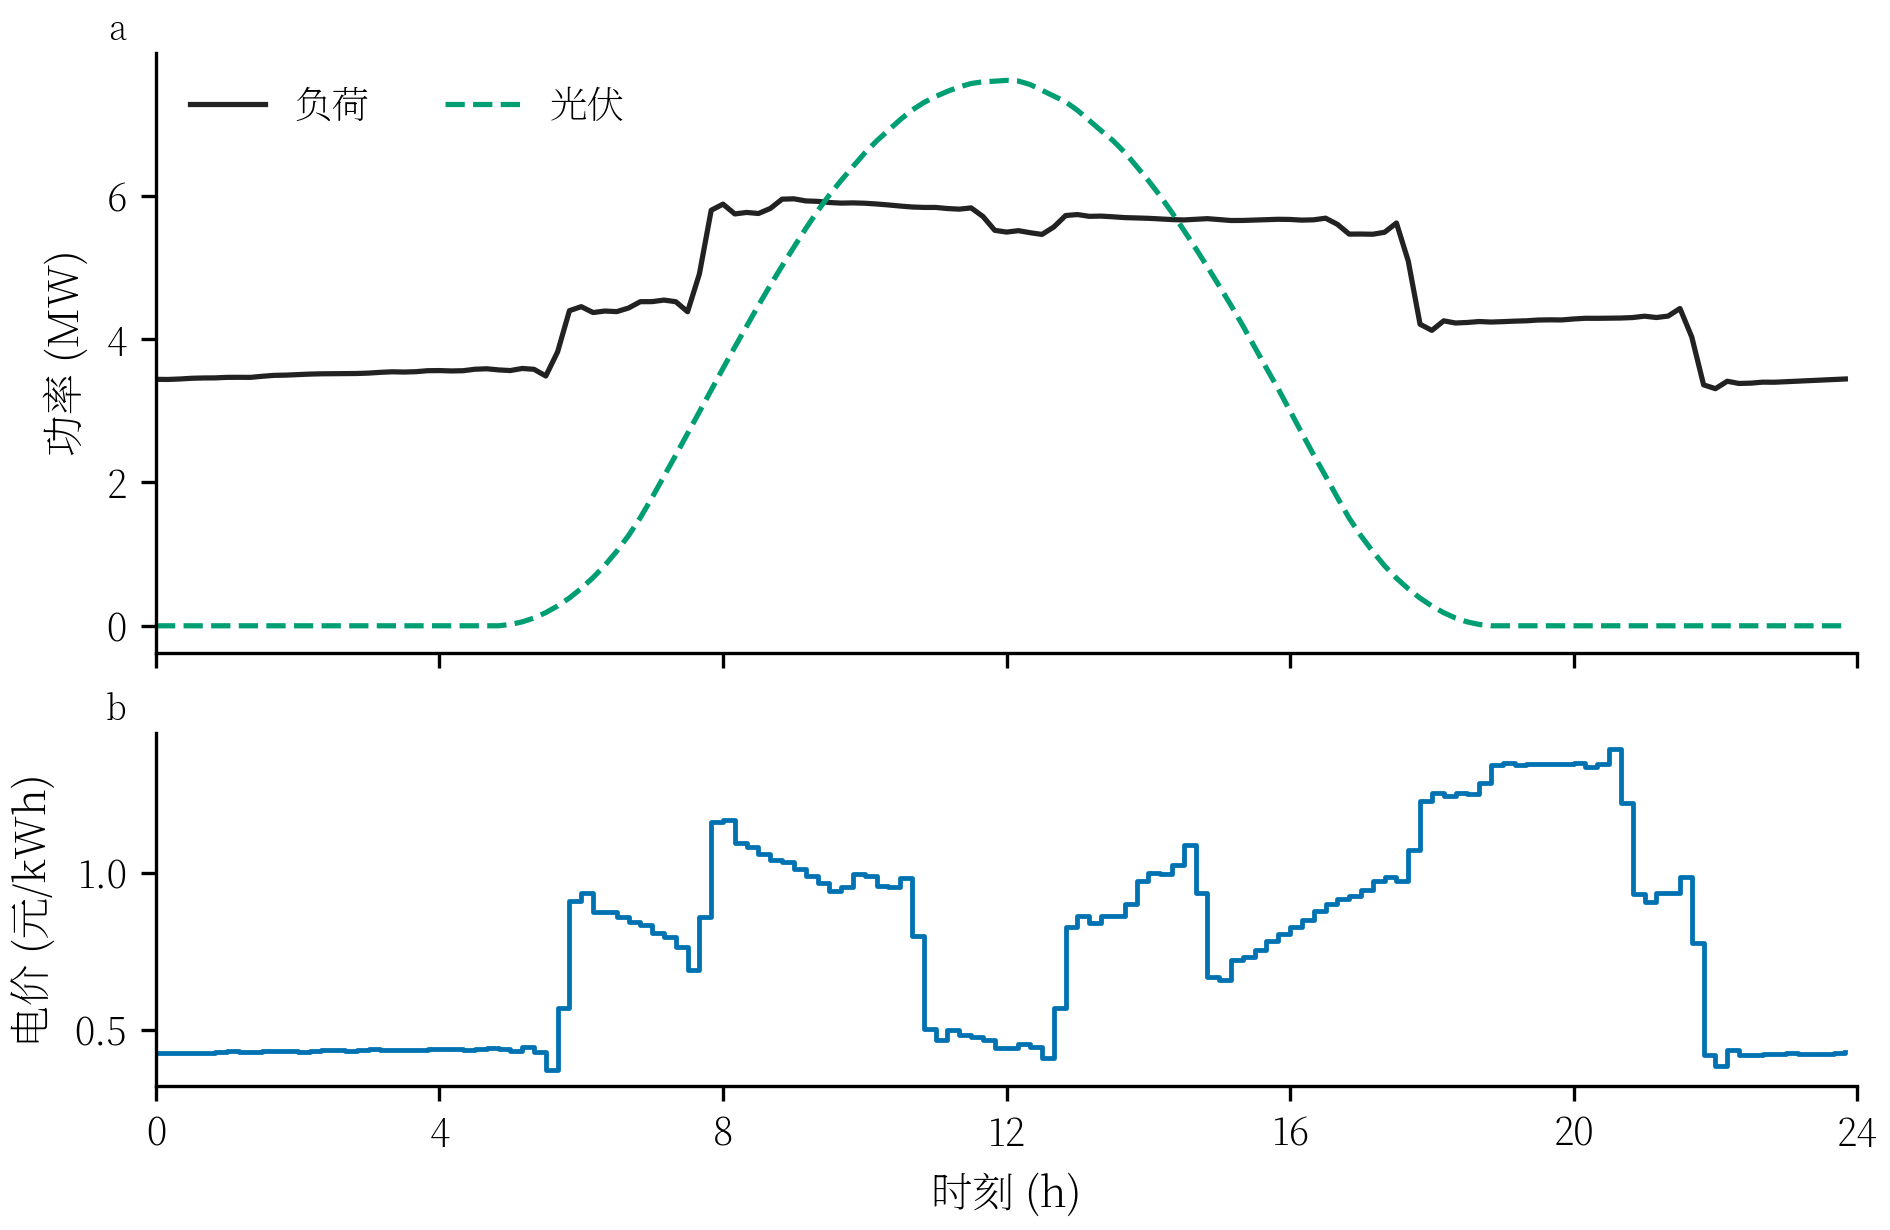
\includegraphics[width=0.96\textwidth]{figs/raw_q1_typical_profiles.png}
  \caption{典型日负荷、光伏与固定电价的日内结构。负荷和光伏峰值并不完全同步，电价阶梯又改变了储能转移能量的价值。}
  \label{fig:q1-raw}
\end{figure}
